%\chapter{computing}

%%%%%%%%%%%%%%%%%%%%%%%%%%%%%%%%%%%%%%%%%%%%%%
\section{Data handling and processing system}

%%%%%%%%%%%%%%%%%%%%%%%%%%%%%%%%%%%%%%%%%%%%%%
\section{LArSoft framework}

%%%%%%%%%%%%%%%%%%%%%%%%%%%%%%%%%%%%%%%%%%%%%%
\section{Event simulation}

%%%%%%%%%%%%%%%%%%%%%%%%%%%%%%%%%%%%%%%%%%%%%%
\section{Event reconstruction algorithms and performance}

description of computing, data handling and on/off-line software\\

may also include reconstruction software description

\subsection{TPC Signal Calibration (Xin)}

In Sec.~\ref{sec:tpc_signal_formation}, the signal formation in TPC
is described. In this section, we describe the procedure of the TPC signal
calibration. As shown in Fig.~\ref{fig:signal_formation}, the goal of TPC 
signal calibration is to recover the number of ionized electrons from the 
digitized TPC signal. 

\subsubsection{Deconvolution Technique}\label{sec:decon}
Deconvolution is a mathematical technique to extract a \textit{real signal}
$S(t)$ from a \textit{measured signal} $M(t_0)$. 
The deconvolution technique was introduced to LArTPC signal processing by 
Bruce Baller in the context ArgoNEUT data analysis~\cite{bruce}. The goal of the 
deconvolution is to ``remove'' the field and electronics response functions 
from the measured signal to recover the number of ionized electrons. This 
technique has the advantages of being robust and fast and is an essential 
step in the overall signal calibration process. 

The measured signal is
modeled as a convolution integral over the real signal $S(t)$ and a
given detector \textit{response function} $R(t,t_0)$ which gives the
instantaneous portion of the measured signal at some time $t_0$ due to
an element of real signal at time $t$.
\begin{equation}\label{eq:decon_1}
M(t_0) = \int_{-\infty}^{\infty}  R(t,t_0) \cdot S(t) \cdot dt.
\end{equation}
If the detector response function only depends on the relative time 
difference between $t$ and $t_0$, we can solve the above equation by 
doing a Fourier transformation on both sides of the equation:
\begin{equation}
M(\omega) = R(\omega) \cdot S(\omega), 
\end{equation}
where $\omega$ is the frequency. In this case, we can derive the signal in the 
frequency domain by taking the ratio of measured signal and the given
response function:
\begin{equation}\label{eq:decon_2}
S(\omega) = \frac{M(\omega)}{R(\omega)}.
\end{equation}
The real signal in the time domain can then be obtained by applying the 
inverse Fourier transformation from the frequency domain. 

The Shockley-Ramo response function $R(\omega)$ does not address
contributions to the measured signal which are due to real world
sources of electrical \textit{noise} from thermal and unwanted transmitting
sources or the approximation in the digitization.
Such contributions to $M(\omega)$ will not be ``divided out'' by the deconvolution.
Worse, because the response function becomes small (see below) at low 
frequencies for the induction planes and at high frequencies for all
planes, the noise components in these frequencies will become
enhanced by the deconvolution.

To address the problem of noise, a \textit{filter function} $F(\omega)$ is
introduced.  Its purpose is to attenuate the problematic noise.  The
addition of this function can be considered an augmentation to the
response function which may in any case be chosen freely as it is a model.  
The two functions are kept distinct for clarity in the notation here.
Equation~\ref{eq:decon_2} is then updated to become
\begin{equation}\label{eq:decon_filt}
S(\omega) = \frac{M(\omega)}{R(\omega)} \cdot F(\omega).
\end{equation}
With a suitable noise model an improved estimator for the signal
$S(t)$ in the time domain can then be found by applying an inverse Fourier 
transform to $S(\omega)$.  Essentially, the deconvolution replaces the field and 
electronics response function with the filter response function. The 
advantage of this procedure shows up on the induction plane where the irregular bipolar 
field response function is replaced by a regular uni-polar response function through
the inclusion of the software filter. 


\subsubsection{Importance of 2D Deconvolution for Induction Planes}
The 1D deconvolution procedure described in the previous section 
works well in dealing with signal in the collection wire plane, but is not 
optimal when applied to signals in the induction wire planes. 
As described in Sec.~\ref{sec:tpc_signal_formation}, the induction plane wire 
signal receives contributions not only from ionization charge 
passing by the wire of interest, but also from ionization charge drifting in 
nearby wire boundaries. In addition, within the boundary of the wire of 
interest the value of the field response function varies appreciably 
and so at small scales the location of the drifting charge relative to the wire 
is important. In this case, Eq.~\ref{eq:decon_1} would naturally expand to 
\begin{equation}\label{eq:decon_2d_1}
M_i(t_0) = \int_{-\infty}^{\infty} \left( R_0 \cdot (t-t_0) \cdot S_i(t) + 
R_1 \cdot (t-t_0) \cdot S_{i+1} (t) + ...\right) \cdot dt,
\end{equation}
where $M_i$ represents the measured signal from wire $i$.  $S_i$ and
$S_{i+1}$ represents the real signal in the boundaries of wire $i$ and
its next neighbor respectively.
The $R_0$ represents the average response function for an ionization
charge passing through the wire boundary of interest.
Similarly, the $R_1$ represents the average response function for an
ionization charge drifting past in the next adjacent wire boundary. One can
easily expand this definition to some number of neighbors by introducing terms up 
to $R_n$.

If we then apply a Fourier transformation on both sides of Eq.~\ref{eq:decon_2d_1},
we have:
\begin{equation}\label{eq:decon_2d_2}
M_i(\omega) = R_0(\omega) \cdot S_i(\omega) + R_1(\omega) \cdot S_{i+1} (\omega) + ...,
\end{equation} 
which can be written in a matrix notation as:
\begin{equation}
\begin{pmatrix}
    M_1(\omega)\\
    M_2(\omega)\\
    \vdots\\
    M_{n-1}(\omega)\\
    M_{n}(\omega)
\end{pmatrix}
=
\begin{pmatrix}
R_0(\omega) & R_1(\omega) & \ldots & R_{n-1}(\omega) & R_n(\omega) \\
R_1(\omega) & R_0(\omega) & \ldots & R_{n-2}(\omega) & R_{n-1}(\omega) \\
    \vdots  & \vdots      & \ddots & \vdots          & \vdots \\
    R_{n-1}(\omega) & R_{n-2}(\omega) & \ldots & R_0(\omega) & R_1(\omega) \\
    R_{n}(\omega) & R_{n-1}(\omega) & \ldots & R_1(\omega) & R_0(\omega) \\
\end{pmatrix}
\cdot
\begin{pmatrix}
    S_1(\omega)\\
    S_2(\omega)\\
    \vdots\\
    S_{n-1}(\omega)\\
    S_{n}(\omega)
\end{pmatrix}
\label{eq:matrix_expansion}
\end{equation}
Now, if we assume that we know response functions (i.e. the matrix $R$), the 
problem converts into deducing the vector of $S$ with the measured signal $M$. 
%
This can be achieved by inverting the matrix $R$. In practice and away
from plane edges the matrix $R$ is taken to be symmetric and its
inversion can again be achieved by the FFT.
%
As this expands the 1D deconvolution (with respect to the time axis)
into a 2D deconvolution (with respect to both the time and wire
axes) similarly we must also expand the filter function to cover
both time and wire dimensions.

A comment on the limitation (or approximation) 
assumed in the 2D deconvolution is needed. As shown in Eq.~\ref{eq:decon_2d_1}, the 
average response functions are used in describing the measured signal. These 
ignore the detailed position dependence of the response function. 
This approximation ignores the fine grained but clear position
dependence in the calculated weighting fields.
However, since we can only measured the signal from any given wire as
a function of time there is no additional information to be used to
resolve the ionization electron distributions within a wire boundary.
This technique can in principle be improved to include the position dependent
response once the local ionization charge distribution is roughly reconstructed. 

\subsubsection{Additional Challenges in Deconvolution}

\begin{figure}[htb]
\centering
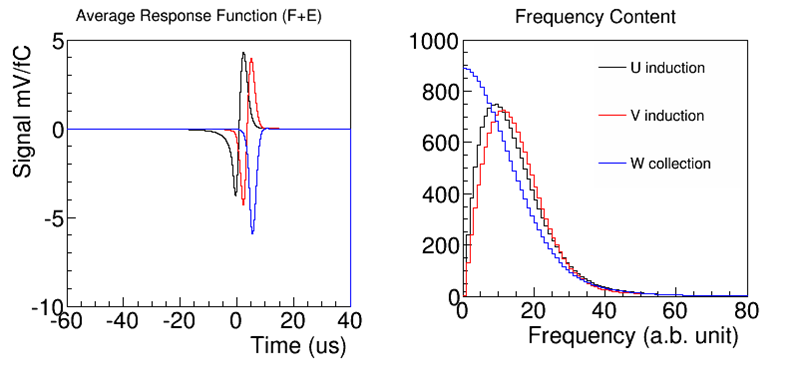
\includegraphics[width=0.95\textwidth]{figures/induction_field_response.png}
\caption{(left) Simulated field response functions for induction (black and red) and 
collection (blue) wires are shown in the time domain. (right) The same are shown in 
the frequency domain.}
\label{fig:induction_field}
\end{figure}

The 1D and 2D deconvolution procedures provide a robust method to extract the ionization
electrons for the collection and induction planes, respectively. 
%
While working well for the collection plane the procedure is still not optimal for the induction plane due to the 
nature of the induction plane signal. Figure~\ref{fig:induction_field} shows the 
field response as simulated by Garfield for induction and collection wire planes and point ionization
electrons. While the field response for the collection wire plane is uni-polar, the field 
response for the induction wire plane is bipolar. 
%
The early, negative half corresponds to the ionization electron moving
towards the wire plane and the late, positive half corresponds
to the ionization electron moving away.
%
The integration of the field response function is close to zero
as the bias wire voltages are applied such that that none of the ionization electrons are
collected. The right panel of Fig.~\ref{fig:induction_field} shows the 
frequency components of the field response. 
%
Since an induction plane field response has a
bipolar shape in the time domain there is a corresponding suppression at low frequency in the frequency 
domain. At zero frequency, the frequency component essentially gives the 
integration of field response function over time and thus should be near zero (again, because no charge is collected).


The suppression of the induction field response at low frequency is problematic for the
proposed deconvolution procedure. First,  the measured signal contains the electronic noise, 
which usually increases at low frequency (the so-called 1/f noise). Therefore, as shown in 
Eq.~\eqref{eq:decon_filt}, the low frequency noise will be amplified in the deconvolution 
process, since the denominator (i.e. the induction field response) is generally small at 
low frequency. This can be seen clearly in Fig.~\ref{fig:decon_example}, where the low frequency noise
is significant. The large low frequency noise would lead to large uncertainty 
in the charge estimation and needs to be dealt with. Three ways to deal with this problem 
are considered. 

\begin{figure}[htb]
\centering
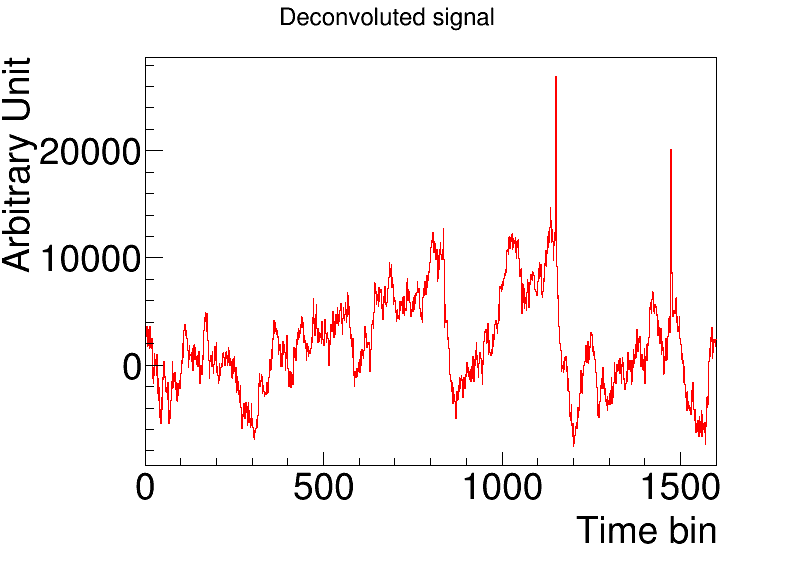
\includegraphics[width=0.8\textwidth]{figures/decon_example.png}
\caption{An example deconvoluted spectrum for the induction plane (simulation).}
\label{fig:decon_example}
\end{figure}

\subsubsubsection{Usage of An Imbalanced Response Function}

As described above, it is the balanced and bipolar nature of the
induction response which leads to it being small at low frequencies
and it is this which then can enhance the noise.
It's natural to then imagine using an intentionally imbalanced field
response in the deconvolution procedure.
As it turns out, this is indeed what has been done initially with the default 1D field response. 
However, the mismatch of the field response function
used in the deconvolution and the actual physical field response 
leads to a distortion of the signal. This in particular is troublesome
near the interaction vertex where multiple tracks are present. 
Therefore, this approach is {\it NOT} acceptable as it introduces large distortions
on the deconvoluted image. On the other hand, one may consider to investigate 
hardware solution of intentionally allow some portion of drifting ionization charge 
to be collected on the induction wires. 

\subsubsubsection{Low-frequency Software Filter}\label{sec:low_freq_filter}

In Eq.~\eqref{eq:decon_filt}, a frequency-domain  filter function is introduced 
to suppress the numerical instability caused by the presence of noise. One can imagine to use this
software filter to suppress the electronic noise at low frequency. This is also 
{\it NOT} acceptable due to large distortion introduced on the signal. To understand this 
point, we recall that the software filter is effectively a smearing function. Figure~\ref{fig:low_f_filter} shows an illustrative 
real signal (left), its convolution with a low-frequency filter (middle), and 
the low-frequency filter itself (right). It is obvious that the signal is strongly 
distorted due to the application of the low-frequency software filter. 

\begin{figure}[htb]
\centering
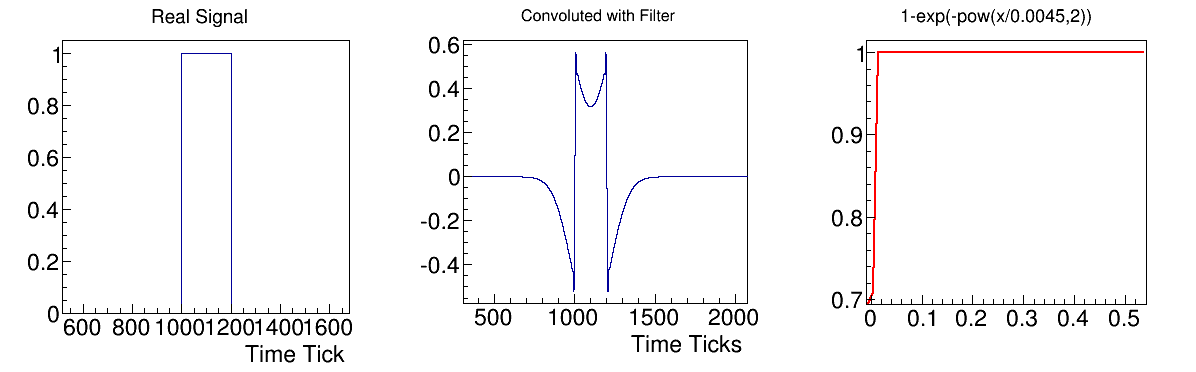
\includegraphics[width=0.95\textwidth]{figures/low_freq.png}
\caption{The impact of the low-frequency filter (right). The unit of the X-axis 
is MHz.  The real signal and the convoluted signal are shown in the left and
middle panel, respectively. A time tick is 0.5 $\mu s$.}
\label{fig:low_f_filter}
\end{figure}

\subsubsubsection{Region Of Interests (ROI) and Adaptive Baseline (AB)}\label{sec:roi_ab}

In the previous two sections, we show that we cannot suppress the low-frequency 
electronic noises with either the intentionally imbalanced response functions nor 
the low-frequency software filter. 
Instead we turn to using two techniques in the time domain: region of interest and 
adaptive baseline. 

The region of interest (ROI) technique
was proposed by Bruce Baller in the context of reducing data size and speeding up the 
deconvolution process. At the same time, the ROI technique can also be used to 
suppressed the low-frequency noise. In order to recognize this point, we consider
a time window with $N$ time ticks.  For MicroBooNE this would be a window of $N\times0.5\mu\mbox{s}$.
The highest frequency that can be resolved with such sampling would be 
1 MHz. The first discrete frequency above zero is be $2/N$ MHz and no result
within the ROI can be sensitive 
to any noise components below this frequency.  Therefore, if we can identify 
the signal region and create a ROI to cover the signal, we can naturally suppress 
the low-frequency noises. 

The adaptive baseline (AB) technique was introduced by 
Mike Mooney in the context of dealing with the ASIC saturation observed in MicroBooNE.
The AB is essentially a local baseline calculated in a given a ROI. However, instead of 
a simple average of the baseline at the start and end points of a ROI, a linear
interpolation is used to correct the baseline. Given the two constraints (start and 
end points of the ROI), the linear interpolation with two degrees of freedom is the best 
that one can achieve to  remove bias in the baseline. 



In the following, we describe various parts used in the signal calibration.

\subsubsection{Calculation of Field Response Function}

The field response is calculated by Garfield~\cite{garfield} in a 22 cm (along the 
field direction) $\times$ 30 cm (along the wire plane direction) region in 2D.  
In the drift direction, the grid plane is labeled as G, the two induction planes wire 
planes are labeled U and V, and the collection plane is W.  The spacing between the wire 
planes is 4.76 mm. The bias voltages of-665 V, -370 V, 0 V, and +820 V for the G, U, V, and 
W planes, respectively, are configured according the operating conditions which ensure 100 \%
    transmission of ionization electrons through the first two induction planes.  
    101 wires with 150 $\mu$m diameter are set on each wire plane with 4.667 (4.79 for collection) mm
    pitch.  A ground plane is placed 1 cm behind the W plane.  The drift
    field is uniform with 500 V/cm. The electron drift velocity as a function of
    electric field is taken from measurements~\cite{Li:2015rqa,lar_property}
    instead of using the default velocity table contained in Garfield. The electron
    diffusion is turned off in the simulation. The field response function then can
    be calculated for each individual wire in the form of induction current 
    (U and V planes) and collection current on (W planes) as a function of time for
    an electron drift which starts from arbitrary position within the region of calculation.
    Figure~\ref{fig:garfield_2d} shows the configuration used in garfield 2D simulation.
The Garfield-simulated response functions are shown in Fig.~\ref{figs:overall_response}.
 The average response function for single electrons within a wire region 
is calculated for the closest wire $R_0$, next adjacent wire $R_1$, and so on. The U and 
V plane responses functions are shown in the middle and right panel of 
Fig.~\ref{figs:overall_response}, respectively.  For induction wire planes, these response 
functions are reasonably balanced as expected.

\begin{figure}[htb]
\centering
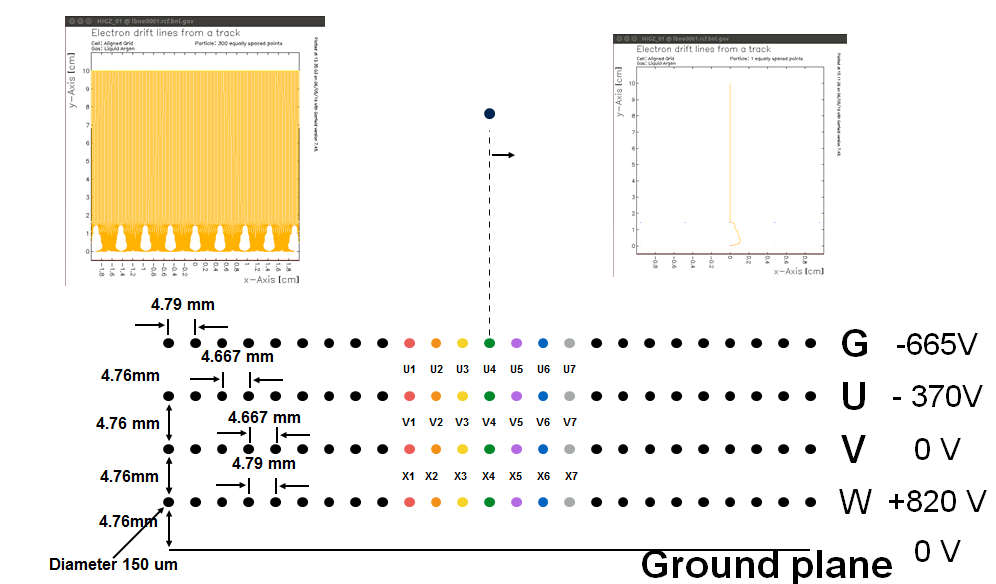
\includegraphics[width=0.95\textwidth]{figures/Garfield_simu.png}
\caption{Description of the Garfield 2D simulation of field response functions.}
\label{fig:garfield_2d}
\end{figure}

\begin{figure}[htb]
\centering
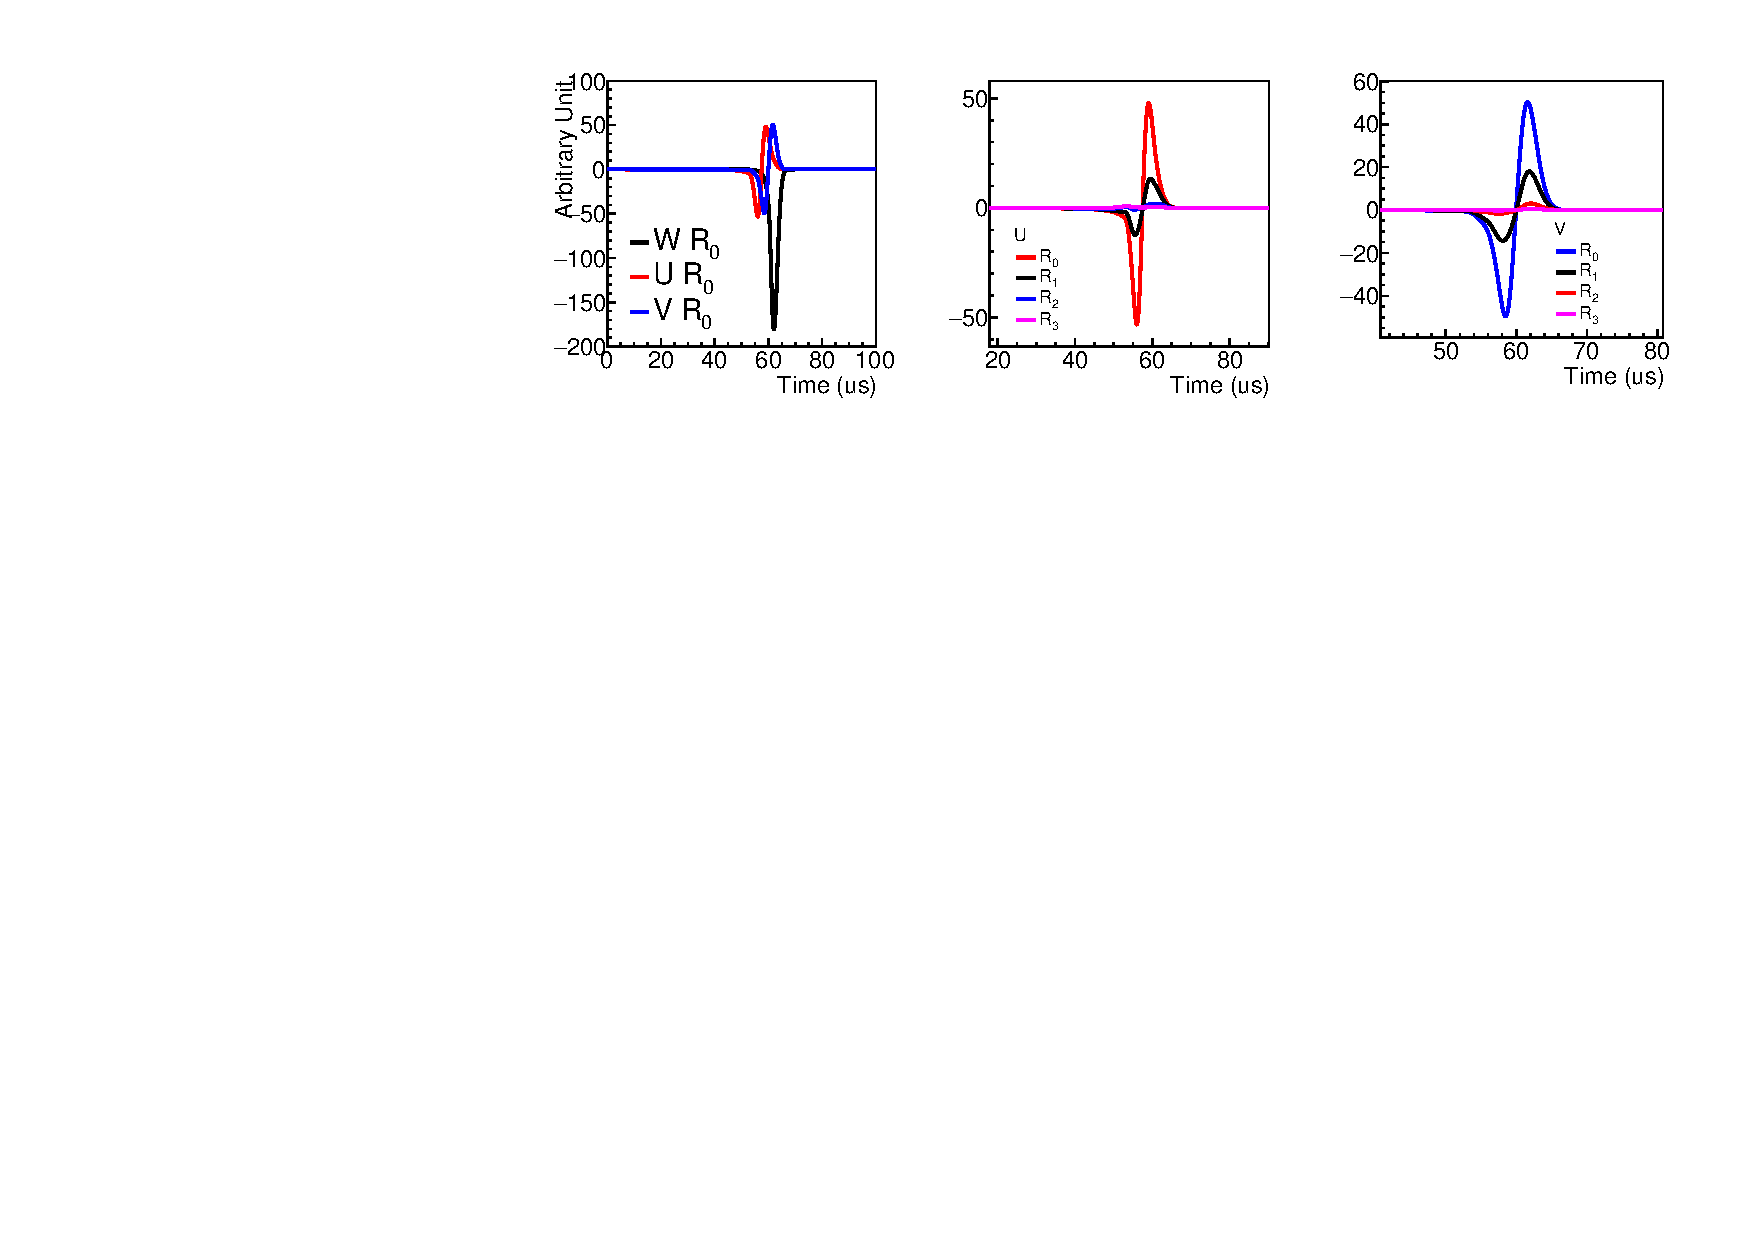
\includegraphics[width=0.95\textwidth]{figures/dune_field_res.pdf}
\caption{The overall response functions, which is the convolution of the
electronics response function (14 mV/fC gain and 2 $\mu$s shaping time) 
and the field response, are shown. }
\label{fig:overall_response}
\end{figure}


\subsubsection{Choice of Software Filter}

We select and implement two types of filters.  The first inspired by the Wiener filter.  It is modified to not suppress
low frequency components.  The second one is the Gaussian filter. While the first one is optimized for 
each wire plane to produce a high signal-to-noise ratio, the second one is optimized and same to all the planes 
to correctly estimate the charge which is independently measured on each of the three planes.  This latter is 
important if all three planes are used for energy measurement and critical for proper application of the
Wire-Cell imaging technique.  In this section, we describe the choice on these software filters.

The standard Wiener noise filter~\cite{wiener} is constructed using the expected 
signal $S(\omega)$ and noise $N(\omega)$ frequency spectra:
\begin{equation}
F(\omega) = \frac{S^2(\omega)}{S^2(\omega) + N^2(\omega)}.
\end{equation}
With this construction, the Wiener filter is expected to achieve the best signal to noise ratio. 
However, applying the Wiener filter to TPC signal processing is problematic. 
%
First, in LArTPC, the TPC signal $S(\omega)$ varies substantially
depending on the exact nature of the event topology.
%
Second, the electronic noise spectrum is a function of the time window
over which it is observed. A longer time window allows for observation
of more low frequency noise components.
%
Third, the induction wire signal spectrum is small at low frequency
and so would be its Wiener filter.  However, as discussed previously, 
a software filter with low-frequency suppression leads to large distortions 
of the signal and is thus not ideal.  

The functional form of the software filter is chosen as:
\begin{equation}
F(\omega) = 
\begin{cases}
e^{- \frac{1}{2} \cdot \left( \frac{\omega}{a} \right)^b} &  \omega >0 \\
0 &  \omega = 0, \\
\end{cases}
\end{equation}
with $a$ and $b$ are two free parameters. 
Note, $b=2$ is basically the Gaussian filter. 
The filter is explicitly zero at $\omega = 0$ in order to remove the DC component in the deconvoluted signal. 
This removes information about the baseline and a new baseline is calculated and restored for the waveform after 
deconvolution. The above functional form of the filter has another advantageous property:
\begin{equation}
lim_{\omega \rightarrow 0} F(\omega) = 1.
\end{equation}
which means the integral of the smearing function is unity, which does not introduce any
extra factor in the overall normalization. The free parameter $a$ and $b$ in the above 
form is determined by matching the tail of Wiener filter at its high frequency side. 
An example of software filter is shown in Fig.~\ref{fig:soft_filter_1}. 

\begin{figure}[!h!tbp]
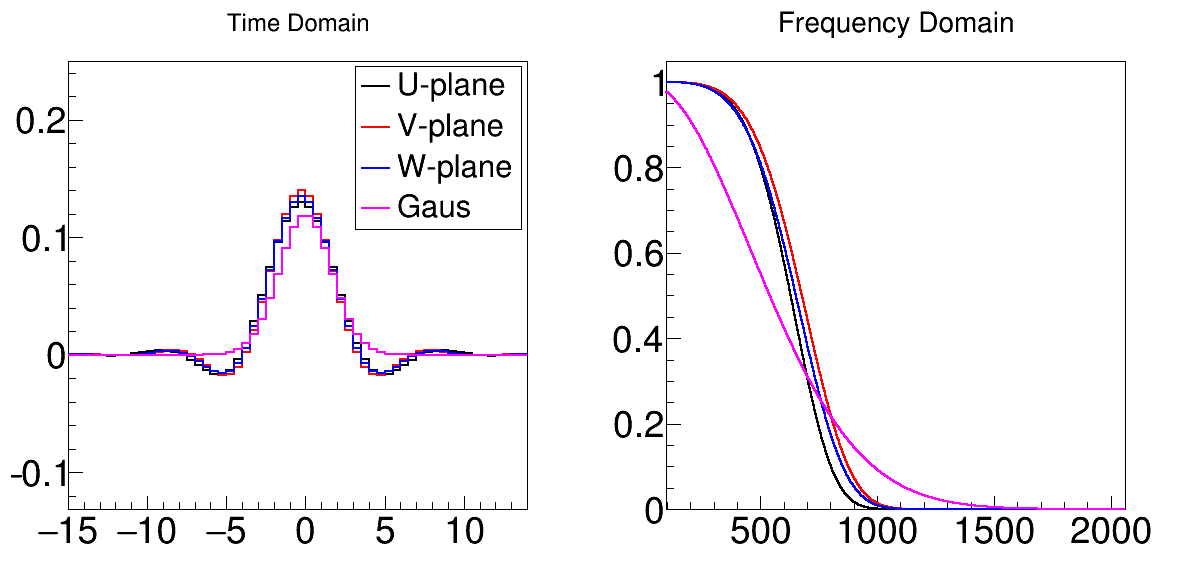
\includegraphics[width=0.8\textwidth]{figures/filter_1.png}
\caption{The Wiener-inspired filter and Gaussian filter used in the 2D deconvolution. 
The time and frequency domain content are shown on the left and right panel, respectively.
The x-axis's unit for the time domain is $\mu$s. For the frequency domain, the number 2000
corresponds to $\sim$0.42 MHz.}
\label{fig:soft_filter_1}
\end{figure}

Beside the high-frequency software filter described above, there is also a low-frequency 
software filter which is used to select ROIs (discussed in the next section). 
The functional form of the low-frequency software filter is 
\begin{equation}
F(\omega) = 1- e^{-\frac{1}{2}\cdot \left( \frac{\omega}{c} \right)^2}.
\end{equation}

\subsubsection{ROI Selection}
The region of interest (ROI) is an important technique to limit the contribution of low-frequency 
electronic noise. The ROI selection was based on the deconvoluted results. Essentially, we perform
three rounds of deconvolution:
\begin{itemize}
\item 1D deconvolution with the imbalanced data-driven field response function (``1D deconvolution'').
\item 2D deconvolution with the balanced Garfield-simulated field response function with a low-frequency filter (``2D deconvolution with low-frequency filter'').
\item 2D deconvolution with the balanced Garfield-simulated field response function without a low-frequency filter (``2D deconvolution'').
\end{itemize}
The first two are used to select ROIs, and the results from the third deconvolution are then used to obtain the final 
deconvoluted results. 

\subsubsection{``Calibration'' of Field Response Function}

In the TPC signal calibration procedure, the response functions are required to be known. 
Assuming the shape of the response functions is known, the relative time 
offsets among the induction U, induction V, and collection W can be calibrated directly 
from the data. Same can be done for the relative normalization 
of the field response function. In this section, we describe the procedure 
that we used to calibrate these time offsets and the relative normalization among field response
functions. 

Wire-Cell imaging determines the likely spatial distribution of
activity in the detector volume which is consistent with the measured
signals.  The distribution is defined on a collection of voxels
filling the volume.  The voxels are shaped as polygonal, right-angled
extrusions.  The two polygonal faces are called ``cells'' and are
parallel to the wire planes.

A cell covers the region near a triple-overlap of one wire from each
plane.  If one imagines a strip with width $\pm\frac{1}{2}$ wire pitch
which runs parallel to the wire and in the wire plane and then further
imagines three strips, one from a wire in each plane, overlapping then
their intersection forms a cell.

The sides of the voxels are parallel to the drift and extend to cover
the distance electrons will drift during one ``time slice'' (chosen to be six
ticks for MicroBooNE with 70 kV drift high voltage.).~\footnote{Space charge 
corrections will lead to a certain warping.}

The measured signal on a wire is subject to a threshold.  For a given
time slice, if the signal is above this threshold the wire is
considered ``hit''.  Likewise, for each time slice, any cell which has
its three associated wires ``hit'' is itself considered
``hit''.~\footnote{In the real world case where some channels do not
  read out, the signal the requirement is relaxed to consider the cell
  hit if at least two wires are hit and the third wire is a known dead 
channel.  This leads to complications such
  as producing artificial cell hits (``ghosting'').}  Given the time
of the hit cell and external information about the initial interaction
time (from the optical detector system), the cell can be projected
into the detector volume along the drift path to provide the location
of the voxel.

The time offsets among the field response functions are therefore calibrated by 
counting the number of cells in the imaging process. For example, a time shift in the 
field 
response function would lead to a time shift in the location of the corresponding hit 
and thus lead to a mist-match hits among three planes, which will reduce the number of 
cells reconstructed. 

One of the unique features of the LArTPC is that each wire plane, be it induction or 
collection provides a measure of the same distribution of ionization electrons.
This 
feature is independent of the initial event topology (i.e. track angle, shower, vertex etc.). 
Therefore, this feature can be used to remove ambiguities made by using wire planes for the 
readout. Using the concept of wire and cell, we can thus write down the following charge 
equation:
\begin{equation}\label{eq:charge}
B\cdot W = G\cdot C.
\end{equation}
Here, $W$ represents a vector of charge measures in wires from all wire planes in a given time slice. 
$B$ is a matrix connecting \textit{merged wires} with single wires~\footnote{A group of ``merged wires'' is formed by collecting together all neighboring hit wires in the time slice.  This is done to reduce the rank of the matrix equation.}.
$C$ is a vector representing the likely amount of ionization electrons in \textit{merged cells} or \textit{blobs}~\footnote{``A group of ``merged cells'' is formed by collecting together all primitive cells which are hit and self-contiguous.}.  $G$ is the geometry 
matrix connecting merged cells and the merged wires. This equation can be expanded into 
a chi-square function:
\begin{equation}\label{eq:chi2}
\chi^2 = \left( B\cdot W - G\cdot C \right)^T V_{BW}^{-1} \left(B\cdot W - G\cdot C\right),
\end{equation}
which also takes into account the uncertainties of the measured charge in 
wires. In particular, $V_{BW} \equiv B \cdot V_{W} \cdot B^{T}$ is the 
covariance matrix describing the uncertainty in (merged) wire 
charges. 

The minimum of the above chi-square function can be found by calculating the 
first derivative
\begin{equation}
\frac{\partial \chi^2}{\partial C} = 0  \rightarrow
G^{T} V_{BW}^{-1} \left(B\cdot W - G\cdot C\right) +
\left(B\cdot W- G\cdot C\right)^{T} V_{BW}^{-1} G = 0,
\end{equation}
and the solution can be written as:
\begin{equation}\label{eq:solution}
C = \left( G^{T} \cdot V_{BW}^{-1} \cdot G \right)^{-1} \cdot G^{T} \cdot V_{BW}^{-1} \cdot B\cdot W.
\end{equation}
The core of the Eq.~\eqref{eq:solution} is the inversion of the matrix 
$G^{T} \cdot V_{BW}^{-1} \cdot G$, which will be referred to as $M$. 
When this matrix can be inverted, the charge
of merged cells can be derived directly. For faked hits (merged cells without 
any ionization charge), the derived charge is likely to be close to zero. For 
real hits (merged cells with ionization charge), the derived charge is like to be
large and close to the true value. On the other hand, if this matrix can not be
inverted, additional assumptions and more advanced techniques are needed to 
derive the solution. The details of these techniques are beyond the scope of this
technote, and will not be discussed here. However, when the charge on the cell is 
solved, we can use them to predict the charge on the wire. Then by comparing the 
the measured charge vs. the predicted charge on the wire, we can calibrate the 
relative normalization of the field response. This is possible because the predicted
charge is calculated assuming all three wire planes are seeing the same amount of 
ionization charge. 



\subsubsection{Metrics in Evaluating TPC Signal Processing}

In order to evaluate the TPC signal processing, which include both the noise filtering and 
the signal calibration, there are two robust metrics that can be used for evaluation 
purpose. 
They are:
\begin{itemize}
\item Equivalent Noise Charge (ENC): \\
  ENC is  basically proportional to the pedestal RMS in terms of ADC, and is a direct 
measure of the noise level in the unit of electrons. It can be used to compare the 
noise levels from different experiments.
\item Deconvoluted Noise Charge after the TPC signal calibration (DNC): \\
The goal of the TPC signal calibration process is to recover the number of ionization 
electrons from the measured TPC signal. With the same procedure, the electronic noise
will also be converted. The unit of these noise is again electrons, which can be compared with 
the expected ionization electrons from energetic charge particles. As described in this technote, 
the DNC depends on the ENC as well as the frequency content of the noise spectrum. It
also depends on the response function used for deconvolution. This is the primary reason 
why the induction plane DNC is much higher than the collection plane DNC. Furthermore, since
we have to rely on ROI and AB techniques to reduce the noise level for the induction plane,
DNC also depends on the time window length of ROI. 
\end{itemize}
Understanding the ENC and DNC for the current-generation experiments and the expected 
performance for the future experiments are important steps to achieve automated event 
reconstruction for LArTPCs.
